\documentclass[11pt]{article}
\usepackage[T1]{fontenc}
\usepackage{lmodern,amsmath,amssymb,amsthm,booktabs,tikz}
\usepackage[letterpaper,margin=1in]{geometry}
\usepackage[hidelinks]{hyperref}
\usepackage{microtype}
\newtheorem{theorem}{Theorem}
\newcommand{\diam}{\operatorname{diam}}
\setlength{\parskip}{3pt}
\title{A cubic counterexample to the diameter bound\texorpdfstring{\\}{} in AutoGraphForge conjecture 5ed263d5}
\author{ProofRush}
\date{26 November 2026 (UTC)}
\begin{document}
\maketitle
\begin{abstract}
A surviving AutoGraphForge conjecture asserts that the diameter of a
nontrivial regular graph is at most one more than its vertex clique cover
number. The cubic graph $G_{14}$ of Brand, Guiduli and Imrich has diameter
eight. We exhibit a partition of its vertices into six cliques and an
independent set of size six. These certificates give a counterexample
with both invariants determined exactly. The negation of the catalogue
statement has been checked in Lean~4 and by the independent Rust kernel nanoda.
\end{abstract}

\section{The conjecture and its setting}
In September 2026 Pastorek described AutoGraphForge, a system that generates
inequalities between graph invariants and tests them on finite graph
datasets~\cite{pastorek}. Its public catalogue retains candidate
\texttt{5ed263d5}~\cite{catalogue}. In the notation of this note the candidate
asks whether every regular finite simple graph $G$ of order at least two satisfies
\begin{equation}
       \diam(G)\ \leq\ \theta(G)+1. \label{eq:source}
\end{equation}
Regularity means that all vertices have the same degree. A clique is a set
of pairwise adjacent vertices. The vertex clique cover number $\theta(G)$
is the fewest cliques whose union is $V(G)$. From any cover one can assign
each vertex to a single clique containing it and discard empty parts.
Thus $\theta(G)$ is also the least size of a clique partition, or equivalently
the chromatic number of the complement. This agrees with the invariant
used by the catalogue~\cite{graphcalc}. On a connected graph the diameter is
the maximum, over vertex pairs, of the length of a shortest path.

\paragraph{Related work.} Brand, Guiduli and Imrich gave a family $G_n$ of
connected cubic graphs in their study of the spectral gap and the maximum
diameter at fixed order~\cite[Definition~1 and Theorem~2]{brand}.
Our witness is their $G_{14}$. A 1976 cubic census already identifies it
as the unique two-bridge cubic graph of order fourteen and tabulates its
diameter~\cite{census}. The application to~\eqref{eq:source} comes from examining a
clique partition of this known graph. The proof below gives all certificates
directly, independently of its diameter extremality.

There is also a short deduction of the negative answer from the older family.
Its member $G_{42}$ consists of two five-vertex end blocks and eight
four-vertex interior blocks. Its diameter is $29$~\cite{brand}.
On a geodesic of length $29$, the alternate edges give fifteen disjoint
two-vertex cliques. The other twelve vertices can be singletons.
This gives $\theta(G_{42})\leq27$, already enough to violate the proposed
bound. The smaller certificate below additionally determines $\theta$
exactly on $G_{14}$.

\begin{figure}[ht]
\centering
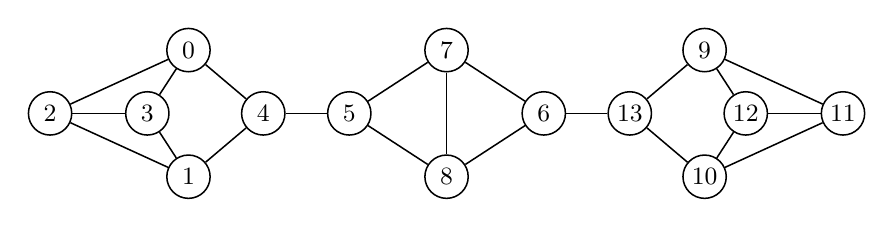
\begin{tikzpicture}[x=.95cm,y=.67cm,
 vertex/.style={circle,draw,fill=white,inner sep=0pt,minimum size=5.5mm,font=\small},
 every path/.style={line width=.55pt}]
\foreach \i/\x/\y in {0/-3.45/1.2,1/-3.45/-1.2,2/-5.3/0,3/-4.0/0,4/-2.45/0,5/-1.30/0,6/1.30/0,7/0/1.2,8/0/-1.2,9/3.45/1.2,10/3.45/-1.2,11/5.3/0,12/4.0/0,13/2.45/0}
  \node[vertex] (v\i) at (\x,\y) {\i};
\foreach \i/\j in {0/2,0/3,0/4,1/2,1/3,1/4,2/3,4/5,5/7,5/8,6/7,6/8,6/13,7/8,9/11,9/12,9/13,10/11,10/12,10/13,11/12}
  \draw (v\i)--(v\j);
\end{tikzpicture}
\caption{The labeled witness. Edges $\{4,5\}$ and $\{6,13\}$ are its two bridges.}
\label{fig:graph}
\end{figure}

\section{The counterexample}
\begin{theorem}\label{thm:main}
There is a connected cubic graph $H$ on fourteen vertices with
$\diam(H)=8$ and $\theta(H)=6$. Consequently conjecture
\texttt{5ed263d5} is false.
\end{theorem}
\begin{proof}
Form three disjoint blocks. In the copy of $K_4$ on $\{0,1,2,3\}$,
subdivide the edge $\{0,1\}$ with the new vertex $4$. In the copy on
$\{9,10,11,12\}$, subdivide the edge $\{9,10\}$ with the new vertex $13$.
Take $K_4$ on $\{5,6,7,8\}$ and delete the edge $\{5,6\}$. Finally add the two
edges $\{4,5\}$ and $\{6,13\}$ as in Figure~\ref{fig:graph}. These edges raise the
degree of each of $4,5,6,13$ from two to three. Every other vertex already
has degree three. The resulting graph is simple and connected.

Within each block any two vertices are at distance at most two.
Joining any two vertices uses at most three blocks and two bridges,
so their distance is at most $2+1+2+1+2=8$ edges. For the reverse bound, every path
from $2$ to $11$ must cross both bridges. Reaching $4$ from $2$,
joining $5$ to $6$, and reaching $11$ from $13$ each require at least
two edges. The path
\[
    2,\ 0,\ 4,\ 5,\ 7,\ 6,\ 13,\ 9,\ 11
\]
attains the resulting lower bound of eight.

The following six sets form a clique partition.
\[
  \{0,2,3\},\quad \{1,4\},\quad \{5,7,8\},\quad
  \{6\},\quad \{9,11,12\},\quad \{10,13\}.
\]
For the matching lower bound, the set $\{0,1,5,6,9,10\}$ is independent.
A clique contains at most one of these six vertices. Hence the clique cover
number of $H$ is exactly six. Inequality~\eqref{eq:source} would give $8\leq7$.
\end{proof}

\section{Formal verification}
The file \texttt{CliqueCoverStatement.lean} quantifies over finite simple
graphs, requires at least two vertices and the existence of a common degree,
and uses Mathlib's diameter and the chromatic number of the complement.
The catalogue's software treats the diameter of a disconnected graph as
undefined. A second declaration explicitly restricts the claim to connected
graphs. The witness satisfies both statements' hypotheses.

In \texttt{RegularCliqueCover.lean} the graph is defined by its edges on
$\mathrm{Fin}(14)$. The diameter proof constructs walks of length at most
four to vertex~$7$. A second labeling changes by at most one per edge and
differs by eight at $2$ and $11$. The complement coloring and its six-vertex
clique give the two bounds on $\theta$. The final declaration
\texttt{RegularCliqueCover.refutes\_5ed263d5} instantiates the universal
claim and derives a contradiction. The theorem with suffix
\texttt{\_on\_domain} also supplies the proof of connectivity.

Lean~4.36.0 accepted the sources against pinned Mathlib. A separate
source-only build exported the theorem and its dependencies. The Rust checker
nanoda accepted all 7,184 exported declarations. The axiom inventory is
\texttt{propext}, \texttt{Classical.choice}, and \texttt{Quot.sound}.
An independent Python calculation computes all pairwise distances by
Floyd--Warshall and the minimum clique partition by subset recursion.

\section{Scope, AI contributions and reproducibility}
The result resolves a single machine-generated candidate. The witness belongs
to an established family. Our search of the source project, related public
code, preprints and bibliographic indexes located no earlier refutation of
this particular candidate. Search coverage is incomplete, and this note
has not undergone external peer review.

ProofRush used the Codex model \texttt{gpt-6.2-astra} in a coordinating
session and three parallel research sessions. The human requester supplied
the research brief and operating conditions. The agents selected the problem,
constructed and checked the witness, searched for earlier results, and wrote
the proof and this note. The research prompts, search decisions, toolchain
versions and machine-checkable proofs are in the
\href{https://github.com/yoshi0703/ProofRush/releases/tag/v1.0.0}{versioned ProofRush archive}. From the project
root run \texttt{python3 experiments/counterexample.py} to reproduce both
invariants. Follow \texttt{REPRODUCE.md} for the complete two-kernel check.

\begin{thebibliography}{9}
\bibitem{pastorek}
J. Pastorek, \emph{AutoGraphForge: Towards Automated Graph Theory Discovery},
2026. \href{https://arxiv.org/abs/2609.03478}{arXiv:2609.03478}.
\bibitem{catalogue}
J. Pastorek, \emph{AutoGraphForge, normalized survivor catalogue}, candidate
\texttt{5ed263d5}, commit \texttt{4d1a8af}, line 2530.
\href{https://github.com/JanPastorek/AutoGraphForge/blob/4d1a8afc99447cacd2328cca20e47b6493e8dbc5/results/survivors_by_touch_normalised.txt\#L2530}{Pinned catalogue entry}.
\bibitem{census}
F. C. Bussemaker, S. \v{C}obelji\'{c}, D. M. Cvetkovi\'{c} and J. J. Seidel,
\emph{Computer Investigation of Cubic Graphs}, report 76-WSK-01,
Technische Hogeschool Eindhoven (1976), pp.~1--2, 6, 8 and the cubic tables.
\href{https://pure.tue.nl/ws/files/1713766/252909.pdf}{Institutional copy}.
\bibitem{brand}
C. Brand, B. Guiduli and W. Imrich, \emph{Characterization of Trivalent
Graphs with Minimal Eigenvalue Gap}, Croatica Chemica Acta \textbf{80}(2)
(2007), 193--201.
\href{https://people.cs.uchicago.edu/~laci/students/guiduli.dir/barry-brand-imrich.pdf}{Author's copy}.
\bibitem{graphcalc}
GraphCalc, \emph{Vertex clique cover number}, source documentation.
\href{https://graphcalc.readthedocs.io/en/stable/_modules/graphcalc/graphs/invariants/classics.html\#vertex_clique_cover_number}{Definition and implementation}.
\end{thebibliography}
\end{document}
